\section{Theoretical foundations}\label{ch:theory}

This section explains the theoretical basis of the ECG system. The system combines
MLII waveform shape, RR timing, and autoencoder residuals in two supervised
Extra Trees ensembles. These components provide complementary information
about beat shape and rhythm.

The explanation follows one beat from measured voltage to the final label.
The equations define the main operations and explain how they contribute to
classification. The three trained components
are a normal-reference autoencoder, a normal-versus-abnormal tree ensemble, and
an abnormal-subtype tree ensemble. The autoencoder learns by changing neural
weights to lower reconstruction error; the tree ensembles learn by choosing
weighted, entropy-reducing splits. These are different forms of training.

\subsection{Why ECG evidence has more than one form}

An ECG is a voltage signal over time. For arrhythmia classification, useful
evidence appears at two related scales. The first is beat-scale morphology:
what the P--QRS--T shape looks like around one R peak. The second is rhythm
timing: when the beat occurs relative to neighbouring beats. The final model
uses both because they answer different questions.

\begin{figure}[H]
\centering
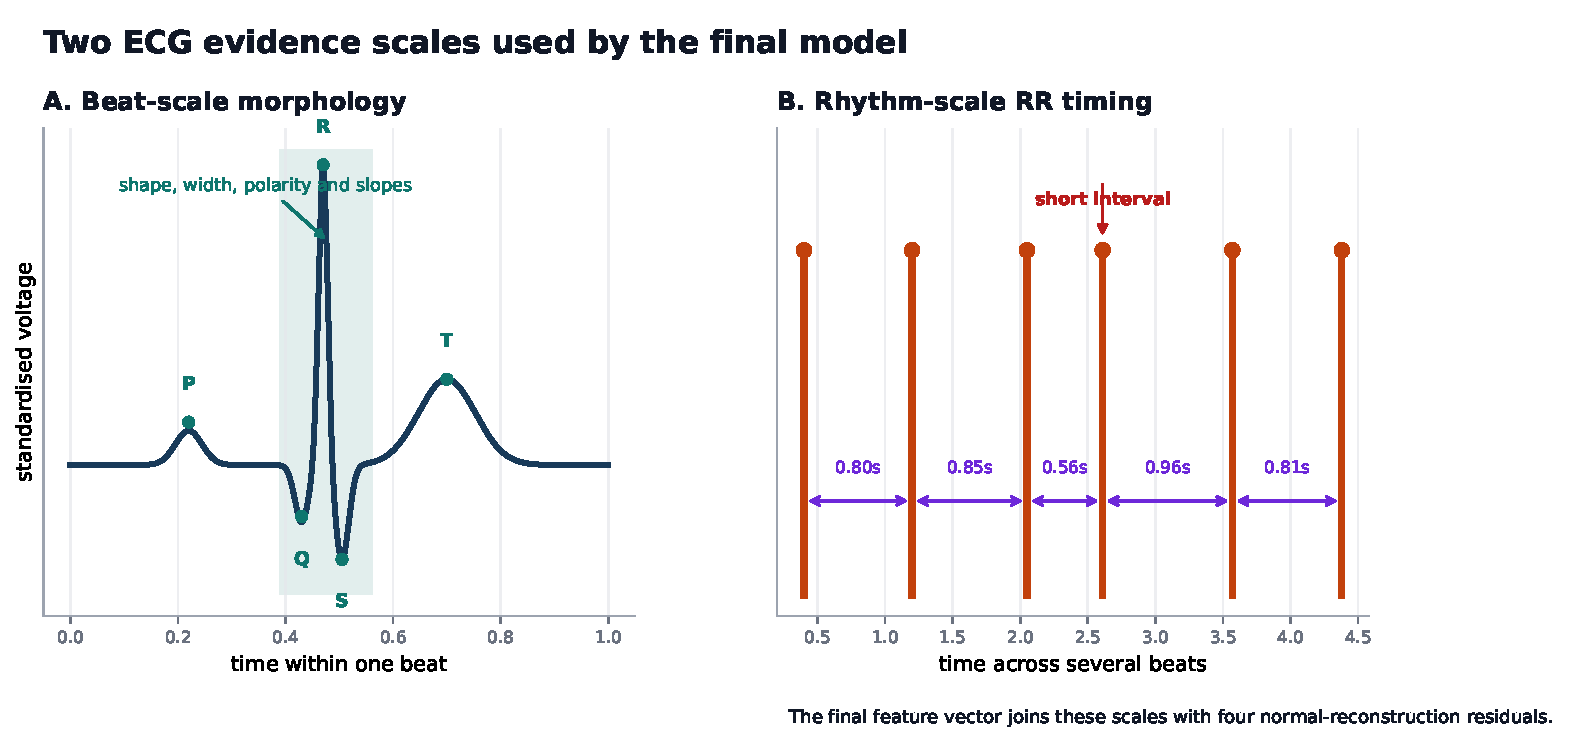
\includegraphics[width=.98\textwidth]{pic/generated/theory_evidence_scales.pdf}
\caption{Two evidence scales used by the final model. Morphology describes the
local shape of a beat; RR timing describes rhythm context around the beat.}
\label{fig:theory-evidence-scales}
\end{figure}

PVC, LBBB, and RBBB can strongly affect QRS shape, width, slopes, and polarity.
PAC and AFib may be easier to detect when timing evidence is also present:
premature beats create short RR intervals, pauses create long RR intervals, and
AFib creates repeated irregularity. Published heartbeat-classification work
also shows the value of combining waveform morphology with heartbeat-interval
features \cite{dechazal2004heartbeat,mousavi2019seq2seq}.

\begin{figure}[H]
\centering
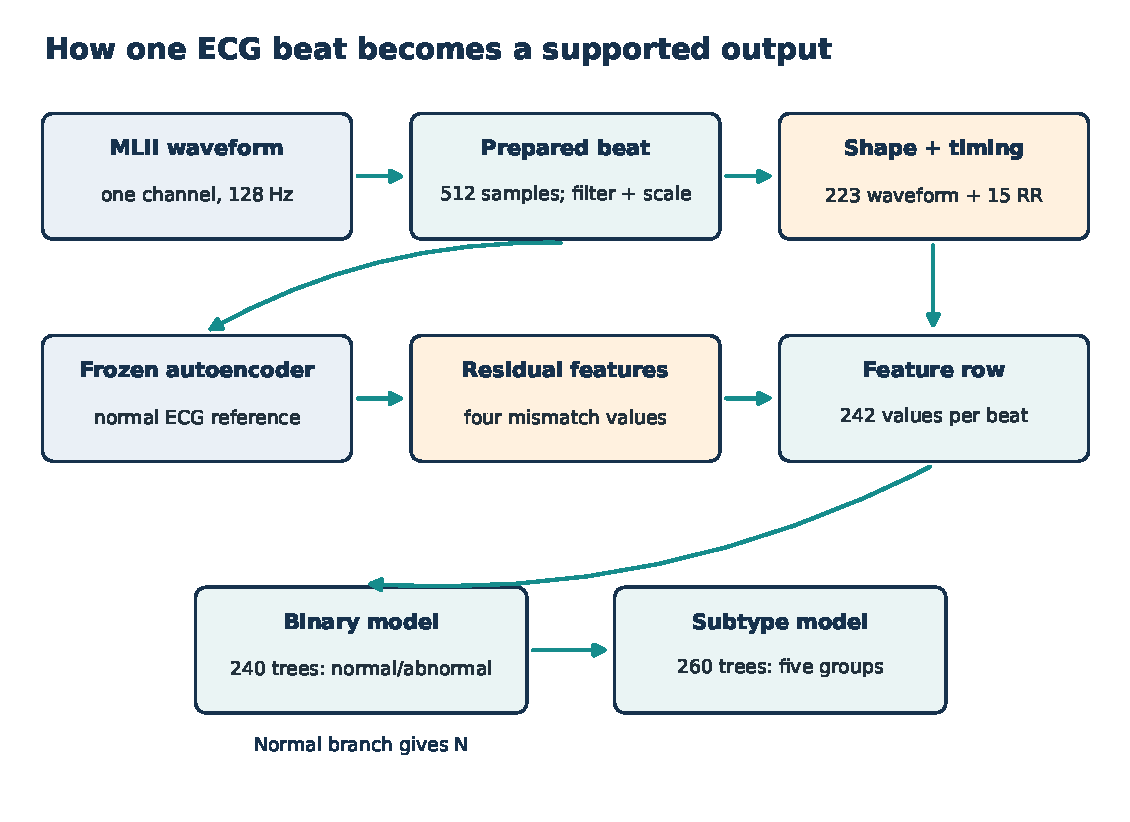
\includegraphics[width=.98\textwidth]{pic/generated/theory_learning_map.pdf}
\caption[Learning map for the final ECG system.]{Reading map for the final system. ECG signal preparation produces one
512-sample window. Three complementary feature groups make one 242-value row.
The frozen autoencoder creates residual features; the two fitted tree
ensembles make the final decision. Labels are used during supervised fitting,
never as input features at prediction time.}
\label{fig:theory-learning-map}
\end{figure}

\subsection{From voltage to a comparable four-second window}

An electrode channel measures a sequence of voltage differences. Sampling at
128 samples per second turns four seconds into $T=4(128)=512$ numbers. The
MITDB waveform is originally sampled at 360~Hz and is resampled to 128~Hz
before beat extraction. Anti-aliasing in the resampling step prevents
high-frequency content from appearing falsely at lower frequencies. The
normal-reference NSRDB channel is already sampled at 128~Hz. Its header calls
the first channel ECG1; the supervised and installed beat input is MLII.
These channel names should not be treated as interchangeable anatomical lead
names \cite{mitdb,nsrdb}.

For supervised examples, an observed R peak is placed at sample 200. Thus a
window contains 200 samples before and 312 samples from that point onward.
The R peak is a useful alignment anchor because many important morphological
changes occur in or near the QRS complex. The normal-reference autoencoder
instead receives consecutive, non-overlapping four-second windows; it does
not need beat labels or R-peak annotations. Figure~\ref{fig:theory-learning-map}
shows where the two streams meet.

The corrected supervised path applies a Butterworth band-pass filter with prototype order four
and 0.5--50~Hz cutoffs to \emph{each} 512-sample window. Forward--backward
filtering removes the phase shift that a one-directional filter would introduce
at an R peak. The lower cutoff attenuates slowly changing baseline, and the
upper cutoff attenuates faster interference. It does not imply that all noise
or motion artifact has disappeared \cite{butterworth1930filter,virtanen2020scipy}.
The NSRDB preparation filters longer recording blocks before making windows;
its archived windows retain their historical scaling, as audited in
Section~\ref{sec:method-real-case}. The local standardisation equation below
describes the corrected supervised MLII path.

If $u_t$ is the filtered voltage in one window, the model receives
\begin{equation}
 x_t=\frac{u_t-\bar u}{s_u+10^{-8}},\quad
 \bar u=\frac{1}{T}\sum_{t=1}^{T}u_t,\quad
 s_u=\sqrt{\frac{1}{T}\sum_{t=1}^{T}(u_t-\bar u)^2}.
 \label{eq:theory-window-zscore}
\end{equation}
Subtracting the window mean removes a local offset. Dividing by its standard
deviation reduces gain differences between recordings. The waveform keeps its
\emph{relative} shape and timing, but absolute millivolt amplitude is no longer
directly available to the model. Flat or non-finite windows are rejected.
Because scaling is calculated inside the current window, later test signal
statistics are not needed when preparing an earlier training beat.

\subsection{Feature extraction theory}

The raw 512-sample MLII window contains more detail than the final tree models
need. Small changes in R-peak alignment or noise can change many raw sample
values. The system therefore converts the window into compact measurements
that keep useful ECG evidence while reducing unnecessary sample-level detail.

\begin{figure}[H]
\centering
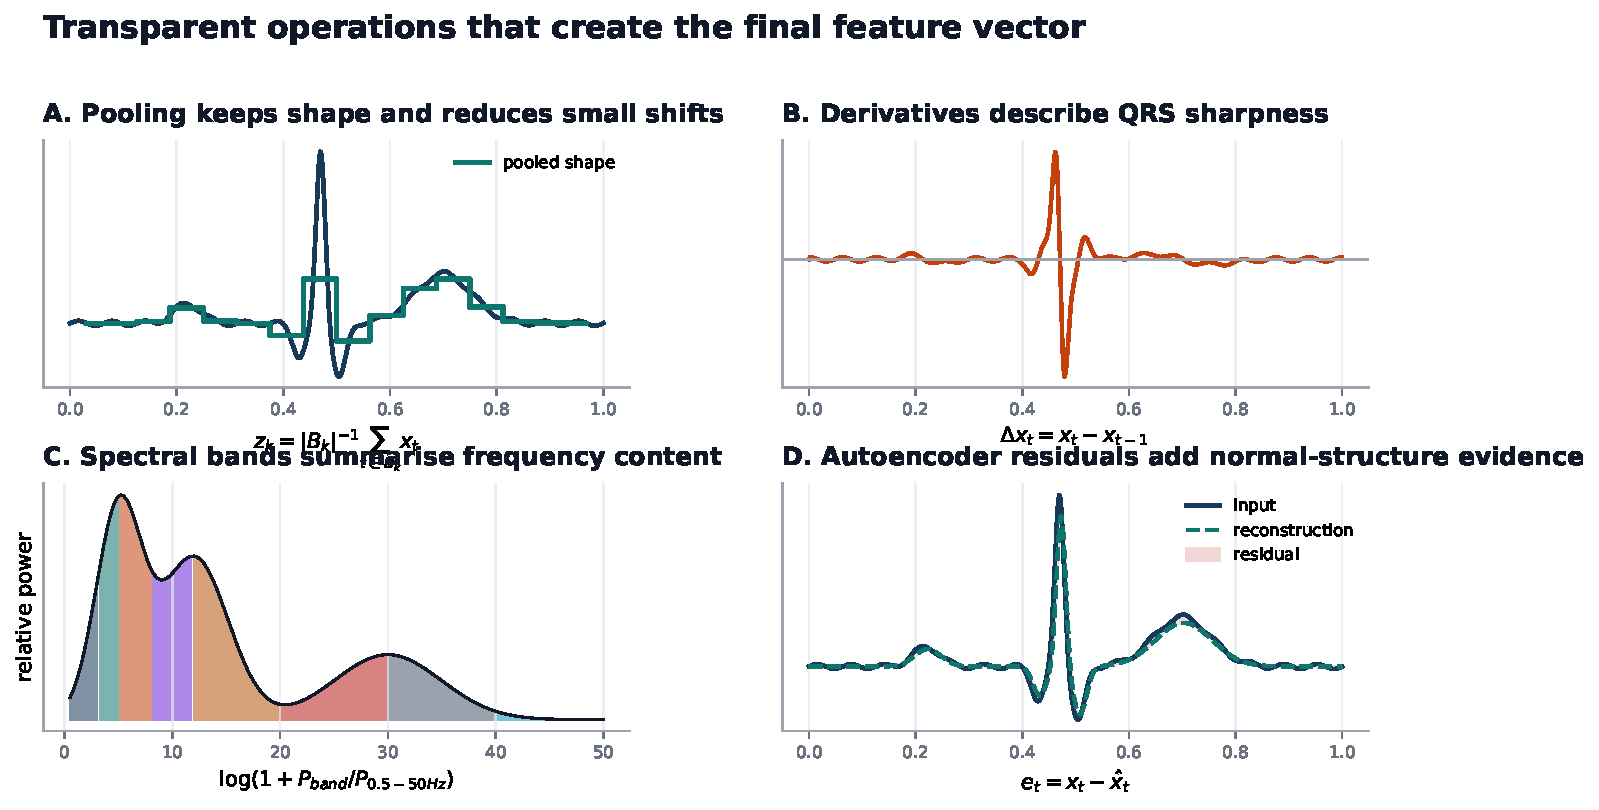
\includegraphics[width=.98\textwidth]{pic/generated/theory_feature_math.pdf}
\caption{Feature-extraction operations behind the final 242-value vector. The
tree models learn from compact numerical evidence, not from raw ECG samples
directly.}
\label{fig:theory-feature-math}
\end{figure}

For a pooled region $B_k$, the pooled value is
\begin{equation}
 z_k=\frac{1}{|B_k|}\sum_{t\in B_k}x_t.
\end{equation}
Pooling keeps the average shape in a small region and makes the representation
less sensitive to a one- or two-sample shift. The final system uses 64
whole-window pooled values and 80 central morphology pooled values.

The derivative
\begin{equation}
 \Delta x_t=x_t-x_{t-1}
\end{equation}
describes how quickly voltage changes. This matters because QRS abnormalities
often change slopes and sharpness. The system keeps 60 pooled derivative values
from the central beat region.

Frequency features describe how signal energy is spread from 0.5 to 50~Hz. For
a frequency band $b$, the relative band feature is
\begin{equation}
 s_b=\log\left(1+\frac{P_b}{P_{0.5-50}}\right),
\end{equation}
where $P_b$ is the power inside the band and $P_{0.5-50}$ is total power in the
ECG band used by the feature extractor. This band-limited view follows the
general ECG idea of keeping physiological content while reducing drift and
high-frequency interference
\cite{kligfield2007standardization,butterworth1930filter}.

Eleven summary statistics add scale, range, energy, skewness, and kurtosis.
Together, the waveform, derivative, spectral, and statistical values form 223
non-RR, non-autoencoder features.

The spectrum is computed with a discrete Fourier transform. For a 512-sample
window, the transform coefficient at frequency index $k$ is
\begin{equation}
 X_k=\sum_{t=0}^{T-1}x_t\exp\!\left(-\frac{2\pi\mathrm{i}kt}{T}\right),
 \qquad P_k=|X_k|^2.
 \label{eq:theory-dft}
\end{equation}
The implementation sums $P_k$ in eight frequency bands between 0.5 and
50~Hz and divides each sum by total power in that range before applying
$\log(1+\cdot)$. The logarithm reduces differences between the relative-power values. These values describe
the distribution of variation by frequency; they are not separate clinical
diagnoses. The eleven statistics include mean, standard deviation, minimum,
maximum, range, mean absolute value, root-mean-square amplitude, derivative
spread and maximum slope, skewness, and excess kurtosis. Skewness describes
asymmetry and kurtosis describes unusually large deviations. The exact count
is $64+80+60+8+11=223$. This count matches the implemented feature vector.

\subsection{RR timing theory}

Let $r_i$ be the time of the R peak of beat $i$. The RR interval is
\begin{equation}
 RR_i=r_i-r_{i-1}.
\end{equation}
RR values describe rhythm. A short interval can suggest a premature beat. A
long interval can suggest a pause. Repeated interval changes support rhythm
irregularity.

The final live system classifies a beat only after it has enough context to
compute the same RR information used in the final experiment. It uses seven
base RR values, including previous RR, next RR, local mean RR, interval ratios,
local coefficient of variation, and heart rate. It then appends eight
history-based values from already completed intervals: median, interquartile
range, median absolute deviation, RMSSD, pNN50, relative range, trend, and
latest interval change.

RMSSD is one example:
\begin{equation}
 \mathrm{RMSSD}=\sqrt{\frac{1}{K-1}\sum_{j=2}^{K}(RR_j-RR_{j-1})^2}.
\end{equation}
The next-RR requirement is important. It delays the streaming decision until the following peak is observed and
allows the same RR features to be used in offline and live processing.

For clarity, the seven base values are previous RR, next RR, mean of up to ten
earlier intervals, previous/mean, next/mean, interval coefficient of
variation, and heart rate $60/RR_{\mathrm{previous}}$. The eight additional
values summarise up to twenty already completed intervals. The interquartile
range is the 75th minus the 25th percentile; median absolute deviation is
the median distance from the median; and $\mathrm{pNN50}$ is the fraction of
successive interval differences exceeding 0.05 seconds. A trend and latest
relative change capture direction. These quantities provide rhythm context
without giving a class label to the model. ``Next RR'' is available only after
the following R peak is observed, so this system makes a delayed beat decision
rather than an instantaneous R-peak decision.

\subsection{Normal-only reconstruction theory}

An autoencoder contains an encoder $f_\theta$ and decoder $g_\phi$. It is
trained to reconstruct a normal ECG window $x$:
\begin{equation}
 \hat{x}=g_\phi(f_\theta(x)), \qquad
 \min_{\theta,\phi}\frac{1}{T}\sum_{t=1}^{T}(x_t-\hat{x}_t)^2.
 \label{eq:ae-objective}
\end{equation}
This follows the representation-learning idea of autoencoders
\cite{hinton2006autoencoder}. The final autoencoder is trained with a
denoising objective: small Gaussian noise is added to the input while the
target remains the clean normal window. Denoising encourages stable structure
instead of exact noise copying \cite{vincent2008denoising}.

\begin{figure}[H]
\centering
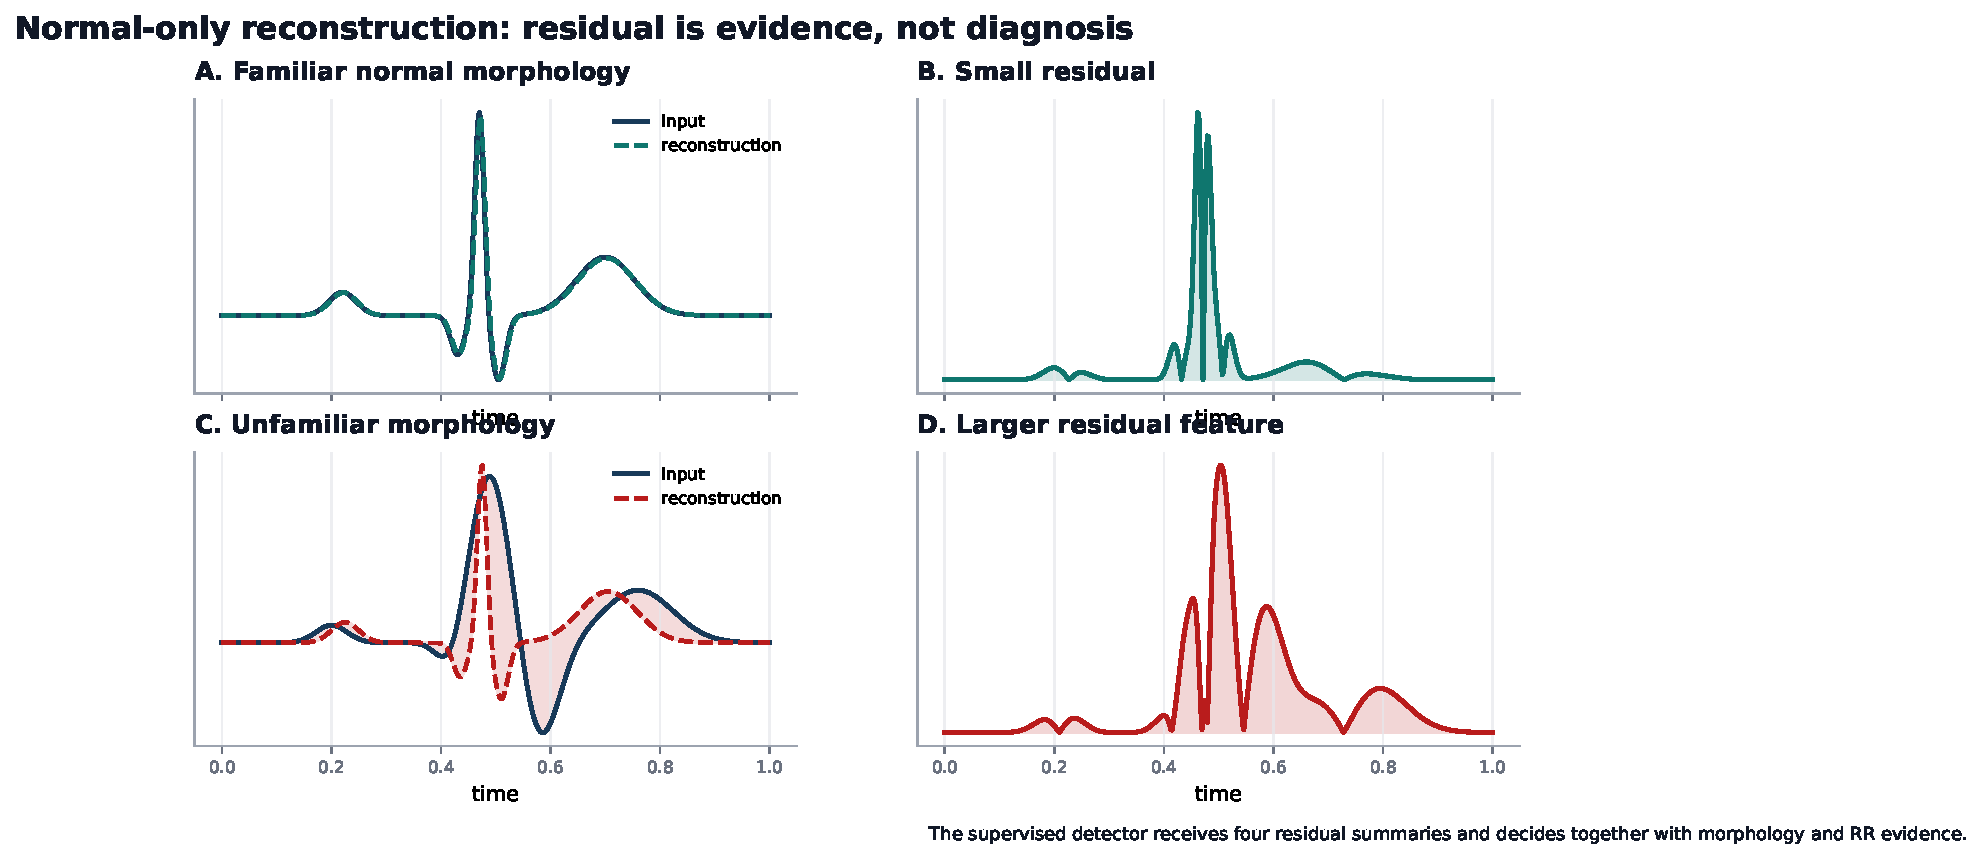
\includegraphics[width=.98\textwidth]{pic/generated/theory_reconstruction_principle.pdf}
\caption{Normal-only reconstruction principle. A larger residual can indicate
novelty, but it is evidence only; the final arrhythmia decision is made by the
supervised hierarchy.}
\label{fig:theory-reconstruction-principle}
\end{figure}

If the autoencoder has learned common normal structure, an unfamiliar or
abnormal beat may be reconstructed less accurately. This is the one-class
anomaly detection idea \cite{chandola2009anomaly}. It is not a guarantee. A
flexible decoder may reconstruct an abnormal waveform well, and noise may
create a large residual for a normal waveform. Therefore, the final system uses
autoencoder mismatch as four supervised input features, not as the final
diagnosis rule.

Let $e_t=x_t-\hat{x}_t$ be the residual. The four residual features are:
\begin{align}
 e_{\mathrm{MAE}} &= \frac{1}{T}\sum_t |e_t|,\\
 e_{\mathrm{MSE}} &= \frac{1}{T}\sum_t e_t^2,\\
 e_{\mathrm{local}} &= \frac{1}{|Q|}\sum_{t\in Q}|e_t|,\\
 e_{\Delta} &= \frac{1}{T-1}\sum_{t=2}^{T}|e_t-e_{t-1}|.
\end{align}
Here $Q$ is the central 240-sample region used by the feature extractor,
defined in Section~\ref{ch:architecture}. The four features measure
whole-window mismatch, squared mismatch, central morphology
mismatch, and residual sharpness. The final architecture appends these four
values to the MLII waveform and RR features.

\subsubsection{What the encoder and decoder actually compute}

The implemented autoencoder is a one-dimensional convolutional network. A
convolution learns a small template and slides it across time. For output
channel $j$ at time $t$, a simplified convolution is
\begin{equation}
 h_{j,t}=b_j+\sum_{c}\sum_{m=0}^{K-1}W_{j,c,m}x_{c,t+m}.
 \label{eq:theory-convolution}
\end{equation}
The learnable numbers $W_{j,c,m}$ and $b_j$ determine which short patterns
activate the channel. A first layer may respond to a steep QRS slope; later
layers can combine such responses over longer time spans. The actual network
uses four encoder blocks to reduce time resolution from 512 to 32 positions
while increasing the channel count to 256. Four decoder blocks restore the
waveform. Figure~\ref{fig:final-ae-layers} gives the verified tensor sizes.

Several architectural functions have distinct purposes. Group normalisation
stabilises intermediate activations. LeakyReLU keeps a non-zero slope for
negative activations, which helps gradients propagate. Residual connections
add a block's input to its transformed output, providing a shorter route for
both signal and gradient flow. Dilation rates 1, 2, 4, and 8 widen the
bottleneck's temporal view without proportionally increasing parameters.
Decoder skip connections pass selected encoder detail forward, scaled by
0.5 in this checkpoint; this helps restore ECG shape but also limits direct
copying. Dropout randomly suppresses activations during fitting to discourage
over-reliance on individual pathways. The last layer is linear so it can
produce both positive and negative standardised voltages
\cite{he2016resnet,ronneberger2015unet,srivastava2014dropout}.

\subsubsection{How the autoencoder lowers reconstruction loss}

Let $x^{(i)}$ be a clean normal window and let
$\epsilon^{(i)}_t\sim\mathcal{N}(0,0.03^2)$ be freshly drawn Gaussian noise.
The training input is $\widetilde x^{(i)}=x^{(i)}+\epsilon^{(i)}$, while the
target is still $x^{(i)}$. For a mini-batch $B$ the actual fitting objective is
\begin{equation}
 \mathcal{L}_{B}(\theta,\phi)=
 \frac{1}{|B|T}\sum_{i\in B}\sum_{t=1}^{T}
 \left[x^{(i)}_t-g_{\phi}(f_{\theta}(\widetilde x^{(i)}))_t\right]^2.
 \label{eq:theory-denoising-loss}
\end{equation}
Squaring makes large reconstruction errors count more strongly. The network
must predict clean structure from a slightly perturbed signal, so simply
copying the input noise is a poor solution. For one output sample, the
derivative of squared error with respect to reconstruction is proportional to
$2(\hat x_t-x_t)$: an output above the target is pushed downward and one below
the target is pushed upward. Backpropagation applies the chain rule through
the decoder and encoder to find the effect of every learned weight
\cite{vincent2008denoising}.

The fitting loop repeatedly performs four operations: clear old gradients,
compute reconstructed windows, backpropagate $\mathcal{L}_{B}$, and take one
Adam step. Adam tracks moving averages of gradients and squared gradients;
schematically, the update is
\begin{equation}
 m_k=\beta_1m_{k-1}+(1-\beta_1)g_k,\quad
 v_k=\beta_2v_{k-1}+(1-\beta_2)g_k^2,\quad
 \theta_{k+1}=\theta_k-\eta\frac{\widehat m_k}
 {\sqrt{\widehat v_k}+\varepsilon}.
 \label{eq:theory-adam}
\end{equation}
Here $g_k$ is the mini-batch gradient, $\eta$ is the learning rate, and hats
indicate bias correction. The same operation updates decoder parameters
$\phi$. Thus ``reducing loss'' means changing millions of network weights in
a direction estimated to reduce expected reconstruction error; it does not
mean manually adjusting a threshold \cite{kingma2015adam}.

\begin{figure}[H]
\centering
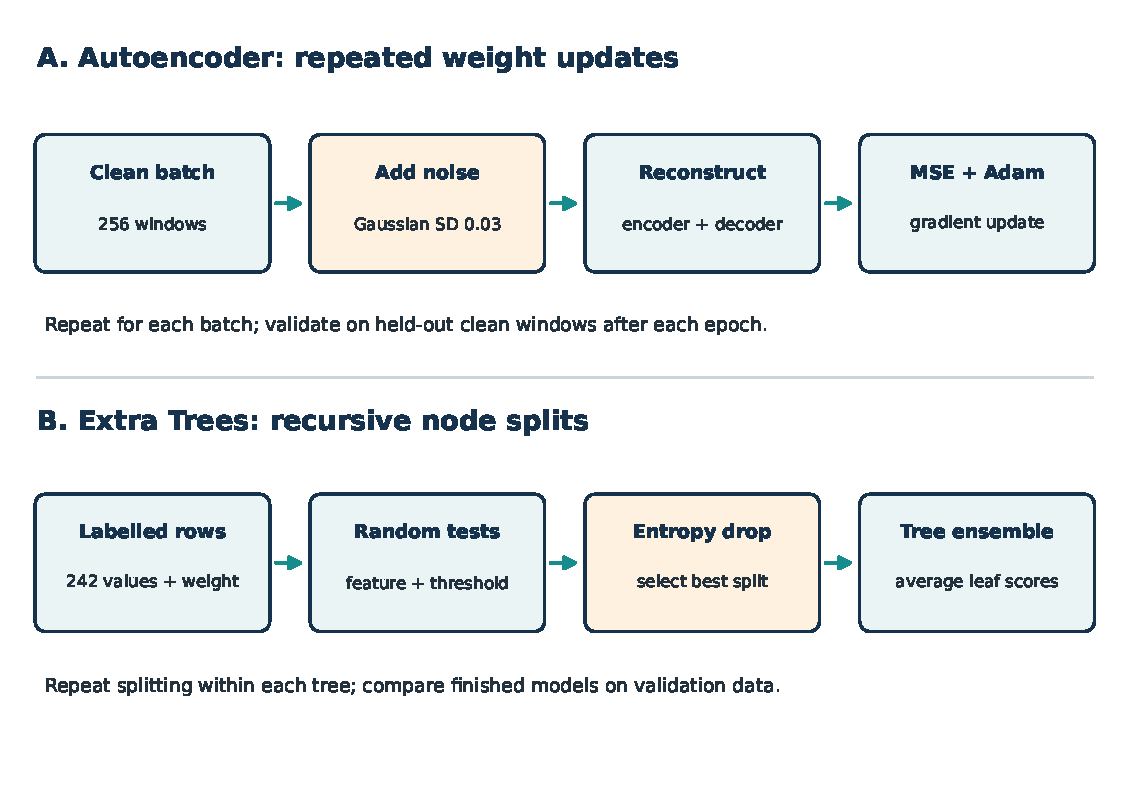
\includegraphics[width=.98\textwidth]{pic/generated/theory_training_mechanisms.pdf}
\caption[Autoencoder and Extra Trees training mechanisms.]{Two distinct learning mechanisms. The autoencoder repeatedly changes
weights from mini-batch reconstruction gradients; an Extra Trees model fixes
each node by comparing randomly proposed splits using weighted entropy. Only
the autoencoder has an epoch-by-epoch reconstruction-loss curve.}
\label{fig:theory-training-mechanisms}
\end{figure}

The implemented training settings and checkpoint-selection rule are specified
in Section~\ref{ch:architecture}. Section~\ref{sec:method-training-inference}
demonstrates the updates numerically and distinguishes the original training
record from the separate real-data teaching demonstration.

\subsection{Hierarchical classification theory}

The hierarchy divides classification into two stages. The first model assigns
a normal or abnormal label. Beats assigned to the abnormal group then enter
the subtype model.

\begin{figure}[H]
\centering
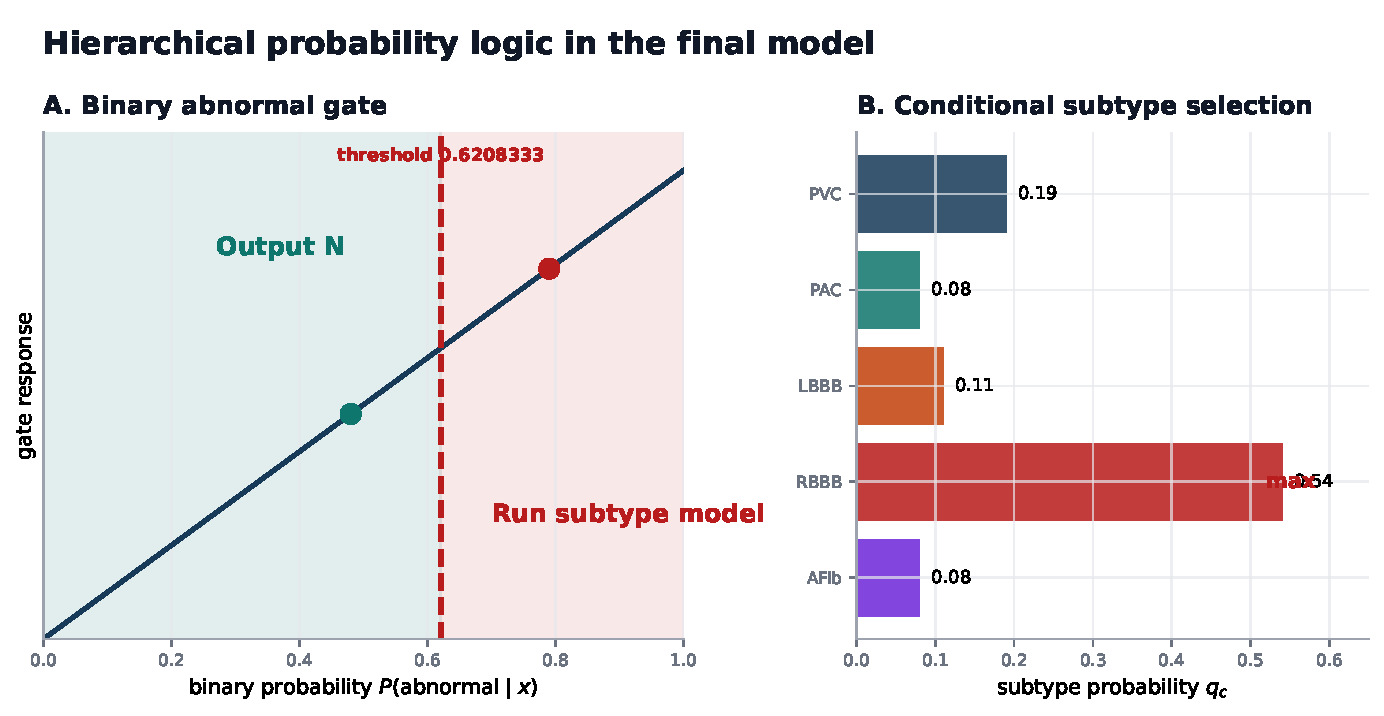
\includegraphics[width=.98\textwidth]{pic/generated/theory_hierarchy_probability.pdf}
\caption{Probability logic of the final hierarchy. The subtype model is
conditional: it is used only after the abnormality gate is passed.}
\label{fig:theory-hierarchy-probability}
\end{figure}

For beat $i$, the binary detector returns an abnormal score $p_i$ from its
242-value feature vector. This score estimates abnormal-class membership
but has not been independently calibrated as a clinical probability.
The final threshold rule is
\begin{equation}
 a_i=\mathbb{1}[p_i>\tau].
\end{equation}
Here $\tau$ is the operating threshold selected using validation data.
If $a_i=0$, the output is N. If $a_i=1$, the subtype model selects the highest
probability among PVC, PAC, LBBB, RBBB, and AFib:
\begin{equation}
 \widehat y_i=\arg\max_{c\in\{1,\ldots,5\}}q_{ic}.
\end{equation}
Here the maximisation already returns an index 1--5. Unsupported abnormal
symbols contribute to binary testing and are excluded from subtype training
and six-class scoring. At inference, every gated beat receives a supported
label. There is no validated unknown-class rejection mechanism.

The tree output is an ensemble score obtained from training-label proportions
in reached leaves. It should not be read as a clinically calibrated disease
probability. In particular, the subtype score $q_{ic}$ is conditional on
taking the abnormal branch; a large $q_{ic}$ does not repair a missed binary
gate. This is why the report evaluates the binary detector, the conditional
subtype model, and the complete six-class decision separately.

\subsection{Why Extra Trees fits this feature design}

The final 242-value vector mixes pooled waveform values, derivatives, spectral
power, signal statistics, RR timing, and autoencoder residuals. Their
relationship to class labels is non-linear. Extra Trees fits this setting by
building many randomised decision trees and averaging their probability
outputs \cite{geurts2006extratrees}.

At a decision-tree node $S$, let $w_i$ be the training weight of beat $i$.
The weighted fraction of class $c$ and its entropy are
\begin{equation}
 p_c(S)=\frac{\sum_{i\in S}w_i\mathbb{1}[y_i=c]}
 {\sum_{i\in S}w_i},\qquad
 H(S)=-\sum_c p_c(S)\log_2 p_c(S),
 \label{eq:theory-weighted-entropy}
\end{equation}
with $0\log_2 0$ defined as zero. Entropy is high when weighted classes are
mixed and zero when a node contains only one class. A proposed split sends
rows to left and right child nodes. Its weighted impurity decrease is
\begin{equation}
 \Delta H=H(S)-\frac{W_L}{W_S}H(S_L)
                 -\frac{W_R}{W_S}H(S_R),
 \qquad W_A=\sum_{i\in A}w_i.
 \label{eq:theory-information-gain}
\end{equation}
For an unweighted toy node with four normal and four abnormal beats, entropy
is one bit. A split putting all normals left and all abnormals right reduces
the two child entropies to zero, giving $\Delta H=1$ bit. Real nodes usually
give a smaller decrease. The tree does not take gradient steps: it selects a
split, partitions the rows, and repeats recursively. Extra Trees randomly
selects candidate features and thresholds at each node, then chooses the
best candidate under this criterion \cite{geurts2006extratrees}.

Each tree ends with leaf nodes. A beat follows feature-threshold questions
from root to leaf, and the leaf's class mixture supplies a score. The ensemble
averages these scores over its trees. Random candidate splits make individual
trees differ; averaging reduces the instability of any one tree. The binary model contains 240 trees and the subtype model contains 260 trees.
Tree count describes ensemble size, whereas an epoch describes one complete
pass through training data in neural-network fitting.

This theory also explains why Extra Trees is suitable for the final data scale.
MITDB contributes many beats but only 45 subject clusters. A very high-capacity
end-to-end neural classifier could learn patient identity instead of robust ECG
rules \cite{zhang2021interpatient}. The Extra Trees hierarchy is still
high-capacity, but it uses transparent tabular evidence and is easier to audit
against the final temporal protocol. This does not mean that tree ensembles are
always better than deep learning.

The binary model learns a normal/abnormal target from all eligible labelled
beats. The subtype model learns only from supported abnormal groups. Both
receive the same feature representation, while the reference labels remain
outside that representation. Section~\ref{sec:method-training-inference}
gives the fitting, weighting, validation, and refitting procedure for each
model. Selection criteria are defined in Section~\ref{ch:method}.

\subsection{Class and patient imbalance theory}

ECG beat datasets are imbalanced in two ways. Some classes are rare, and some
patients contribute many more beats than others. Without weighting, a model can
mostly learn common normal beats or a few large records.

The final training code uses record-aware class weights. For class $c$ in
subject cluster $r$, the weight is proportional to
\begin{equation}
 w_{cr}=\frac{1}{n_c}
 \left(\frac{n_c}{R_c n_{cr}}\right)^\alpha,
 \label{eq:record-weight}
\end{equation}
where $n_c$ is total support for class $c$, $R_c$ is the number of subject clusters
containing class $c$, and $n_{cr}$ is the number of class-$c$ beats in subject cluster
$r$ (records 201 and 202 are combined). Weights are normalised to mean one
and clipped to $[0.05,20]$. The first factor supports class balancing; the second factor reduces
domination by a single record. The exponent $\alpha$ controls how strongly
record balancing is applied and is selected in validation. Class-balanced
learning is important when rare classes would otherwise have little influence
\cite{cui2019classbalanced}.

\subsection{Temporal patient adaptation theory}

ECG morphology contains patient-specific information such as body geometry,
electrode placement, baseline QRS shape, conduction pattern, and background
rhythm. If earlier labelled ECG from a patient is available during development,
the model can adapt to that patient's baseline. This shared patient information can make classification easier than it would
be for a patient whose ECG was absent from development.

This is the theory behind the final temporal-holdout design. It is useful for
monitoring after a labelled calibration period, but it changes the claim. The
final result is a known-patient temporal-continuation result. It should not be
reported as unseen-patient generalisation unless a patient-disjoint experiment
is run. The 16-beat boundary gap reduces direct overlap at the split boundary,
but it does not remove shared patient identity.

\subsubsection{Why training, validation, and testing have different jobs}

Training data changes model parameters: neural weights for the autoencoder,
and split rules and leaf scores for each tree ensemble. Validation data
chooses among checkpoints, tree settings, and the binary operating threshold.
The temporal test then estimates performance after those choices are fixed.
If test labels were used to choose the best threshold, its reported score
would be optimistically biased. In this final rerun, the test did not select
the threshold or candidate, but its labels had been seen during earlier
development. The result is therefore a retrospective known-patient estimate,
not a fresh confirmatory test. Figure~\ref{fig:method-workflow} shows the
chronological allocation and boundary gaps.

\subsection{Validation theory}

Beat-level accuracy alone is not enough. If one patient contributes 2,000
beats, those beats are related. They are not equivalent to 2,000 independent
patients. The final validation therefore reports beat metrics and also uses
subject-clustered uncertainty.

\begin{figure}[H]
\centering
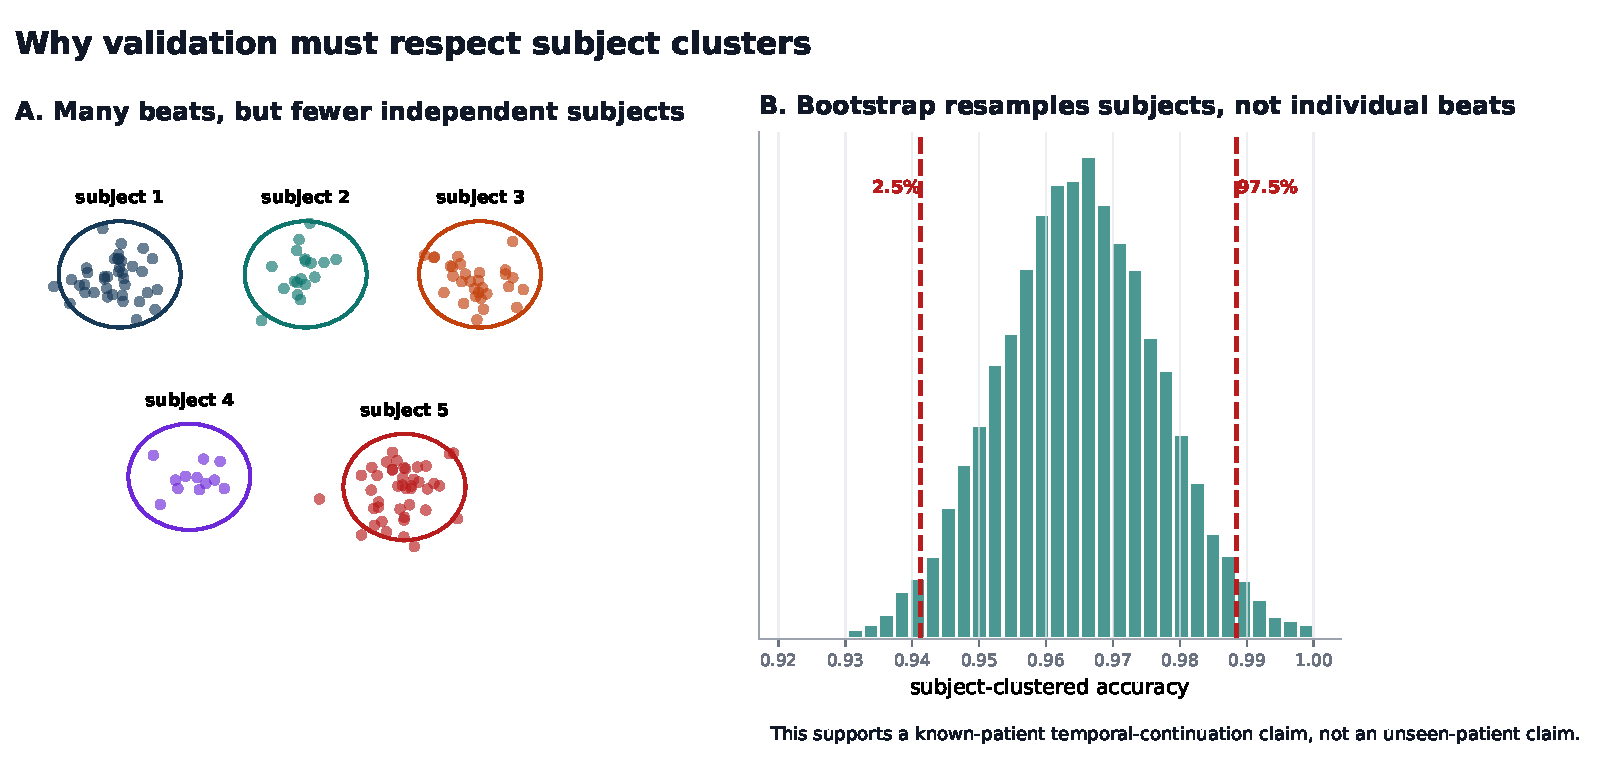
\includegraphics[width=.98\textwidth]{pic/generated/theory_validation_units.pdf}
\caption{Theoretical reason for subject-clustered validation. Clustered
resampling prevents one long record from being treated as many independent
people.}
\label{fig:theory-validation-units}
\end{figure}

Balanced accuracy gives equal weight to class recalls, so normal beats cannot
hide poor abnormal recall. Macro F1 gives each class equal importance, so a
failure on a rare class is visible. Precision--recall style measures are also
important under class imbalance \cite{saito2015pr}. For confidence intervals,
the final experiment resamples complete subject clusters rather than individual
beats, following the general diagnostic-statistics principle that clustered
data need clustered analysis \cite{rutter2000clustered}.

A confusion matrix counts every true/predicted class pair, making aggregate
accuracy easier to interpret. Section~\ref{ch:method} defines the metrics and
bootstrap procedure. Subject-clustered uncertainty does not correct for prior
test exposure or establish generalisation to patients absent from development.

\subsection{Summary of the theoretical framework}

\begin{table}[H]
\centering
\caption{How the theory maps to the implemented final system.}
\label{tab:theory-system-alignment}
\begin{tabular}{>{\raggedright\arraybackslash}p{4.2cm}>{\raggedright\arraybackslash}p{9.0cm}}
\toprule
Theory concept & Implemented in the final system\\
\midrule
Beat-scale morphology & 512-sample MLII window with pooled full-window,
central, and derivative features\\
Rhythm timing & 15 RR features; live scoring waits until next-RR context is
available\\
Normal-only reconstruction & frozen NSRDB autoencoder supplies four residual
features\\
Hierarchical probability & 240-tree binary gate first; 260-tree subtype model
only for gated abnormal beats\\
Class/patient imbalance & record-aware class weighting with validation-selected
record-power parameter\\
Temporal adaptation & earlier MLII timeline trains/selects the model; final
20\% of accepted beats is tested\\
Subject-aware uncertainty & subject-clustered bootstrap over 45 clusters, with
records 201 and 202 treated as one cluster\\
\bottomrule
\end{tabular}
\end{table}
